\documentclass[titlepage,12pt]{article}
\usepackage{geometry}[1in]
\usepackage{multirow}
\usepackage{nth}
\usepackage{amsmath}
\usepackage[section]{placeins}
\usepackage{graphicx}
    \graphicspath{{media/}} 
\usepackage{tikz}
\usepackage{framed}
\usepackage{float}
\usepackage[
    colorlinks,
    linkcolor=black,
    citecolor=black,
    urlcolor=blue
]{hyperref}
\usepackage{subcaption}


\setlength{\parskip}{1em}
\setlength{\parindent}{0em}

\title{Investigating the motion of a gravity car}
\author{Michalis Pardalos}
\date{}

\begin{document}

\maketitle
\section{Experimental Design}

\subsection{Focus Question}

How does the weight connected to a gravity car affect the distance it travels

\subsection{Hypothesis}

The distance travelled will increase with the mass attached to the car, up to a maximum
value.

\subsection{Theory}

Let $A$ the point at which the car starts, $B$ the point at which at the weight touches the
base of the car, and $C$ the point at which the car stops. Also, let $M$ the mass of the
whole car, $m$ the mass of the weight attached to the car, $h$ the height from which the
height is dropped, $r$ the radius of the wheels, $r_a$ the radius of the axle attached to
the wheels, and $m_w$ the mass of one of the wheels.

The distance $AB$ depends on $h$, $r$, and $r_a$. When the weight falls by $h$, the axle
will rotate by the same angular displacement $\theta$ as the wheels, 
%
\begin{align*}
    AB = \frac{r}{r_a} h
\end{align*}
%
Next, the distance $BC$ depends on the velocity $v_B$ with which the car reaches $B$ as well
as the friction $f$ which is applied to the car. 

Ignoring the energy lost to heat, by conservation of mechanical energy,
%
\begin{align*}
    \underbrace{\frac{1}{2}(M+m)v_B^2}_{\text{Translational Kinetic Energy of Car}} +
    \underbrace{4\cdot\frac{1}{2}I\omega^2}_{\text{Rotational Kinetic Energy of Wheels}} &=
    \underbrace{mgh}_{\text{Gravitational Potential Energy of Weight}}
\end{align*}
%
The moment of inertia of each wheel is $\frac{1}{2}m_wr^2$, and the angular velocity of each
wheel is $\frac{u_b}{r}$. Substituting these values gives:
%
\begin{align*}
    \frac{1}{2}(M+m)u_B^2 + 2I\omega^2                          &= mgh \Rightarrow \\
    \frac{1}{2}(M+m)u_B^2 + 2\frac{1}{2}m_wr^2(\frac{u_b}{r})^2 &= mgh \Rightarrow \\
    \frac{1}{2}(M+m)u_B^2 + \frac{1}{r^2}u_b^2 &= mgh
\end{align*}
%
Solving for $u_B$, this becomes:
%
\begin{align*}
    u_B = \sqrt{\frac{2mgh}{M+m_w+m}}
\end{align*}
%
Then, $BC$ will equal $\frac{u_B^2}{2a_f}$ where $a_f$ is the acceleration of the car due to
friction. $a_f$ equals $\frac{\mu M g}{M} = \mu g$, So, 
%
\begin{align*}
    BC &= \dfrac{u_B^2}{2a_f} = \dfrac{\dfrac{2mgh}{M+m_w+m}}{2\mu g}
                             = \dfrac{mh}{\mu(M+m_w+m)} \\
       &= \frac{h\cdot \mathbf{m}}{\mu(M+m_w) + \mu \cdot \textbf{m}}
\end{align*}
%
The complete distance covered $S=AB+BC$ covered by the car will, therefore be: 
%
\begin{framed}
    \begin{equation} \label{eq:s_formula}
    \begin{aligned}
        S = \frac{r}{r_a}h + \frac{h\cdot \mathbf{m}}{\mu(M+m_w) + \mu \cdot \textbf{m}}
    \end{aligned}
    \end{equation}
\end{framed}
%
This means that the distance covered by the car will continuously increase with $m$,
asymptotically approaching $\frac{r}{r_a}h + \frac{h}{\mu}$

\subsection{Variables}

\begin{table}[h!]
    \centering
    \label{my-label}
    \begin{tabular}{l|l|p{5cm}}
        Variables identified & Type of variable   & Treatment\\
        \hline
        \hline
        Mass on string       & Independent        & Increased in 20g increments\\
        \hline
        Distance covered     & Dependent          & 5 measurements taken for each weight increment\\
        \hline
        Car                  & Controlled         & The car remains the same in all aspects for each measurement\\
        \hline
        Tire width           & Controlled         & The same $21.97mm$ tires used for all measurements\\
        \hline
        Height               & Controlled         & The weight is always dropped from the same height from the platform of the car\\
    \end{tabular}
\end{table}
\FloatBarrier

\subsection{Apparatus \& Materials}

\begin{itemize}
    \item Lego pieces (for making the gravity car)
    \item Measured weights and weight holder
    \item String
    \item Data Logger
    \item Ultrasonic distance sensor
    \item Laptop
\end{itemize}

\subsection{Procedure}

\subsubsection{Construction of the gravity car}

\begin{figure}[H]
    \hspace*{-1.3in}
    \begin{subfigure}{.5\paperwidth}
        \centering
        \includegraphics[width=.5\linewidth]{car_diagram.jpg}
        \caption{Diagram of gravity car}
        \label{fig:car_diagram}
    \end{subfigure}%
    \begin{subfigure}{.5\paperwidth}
        \centering
        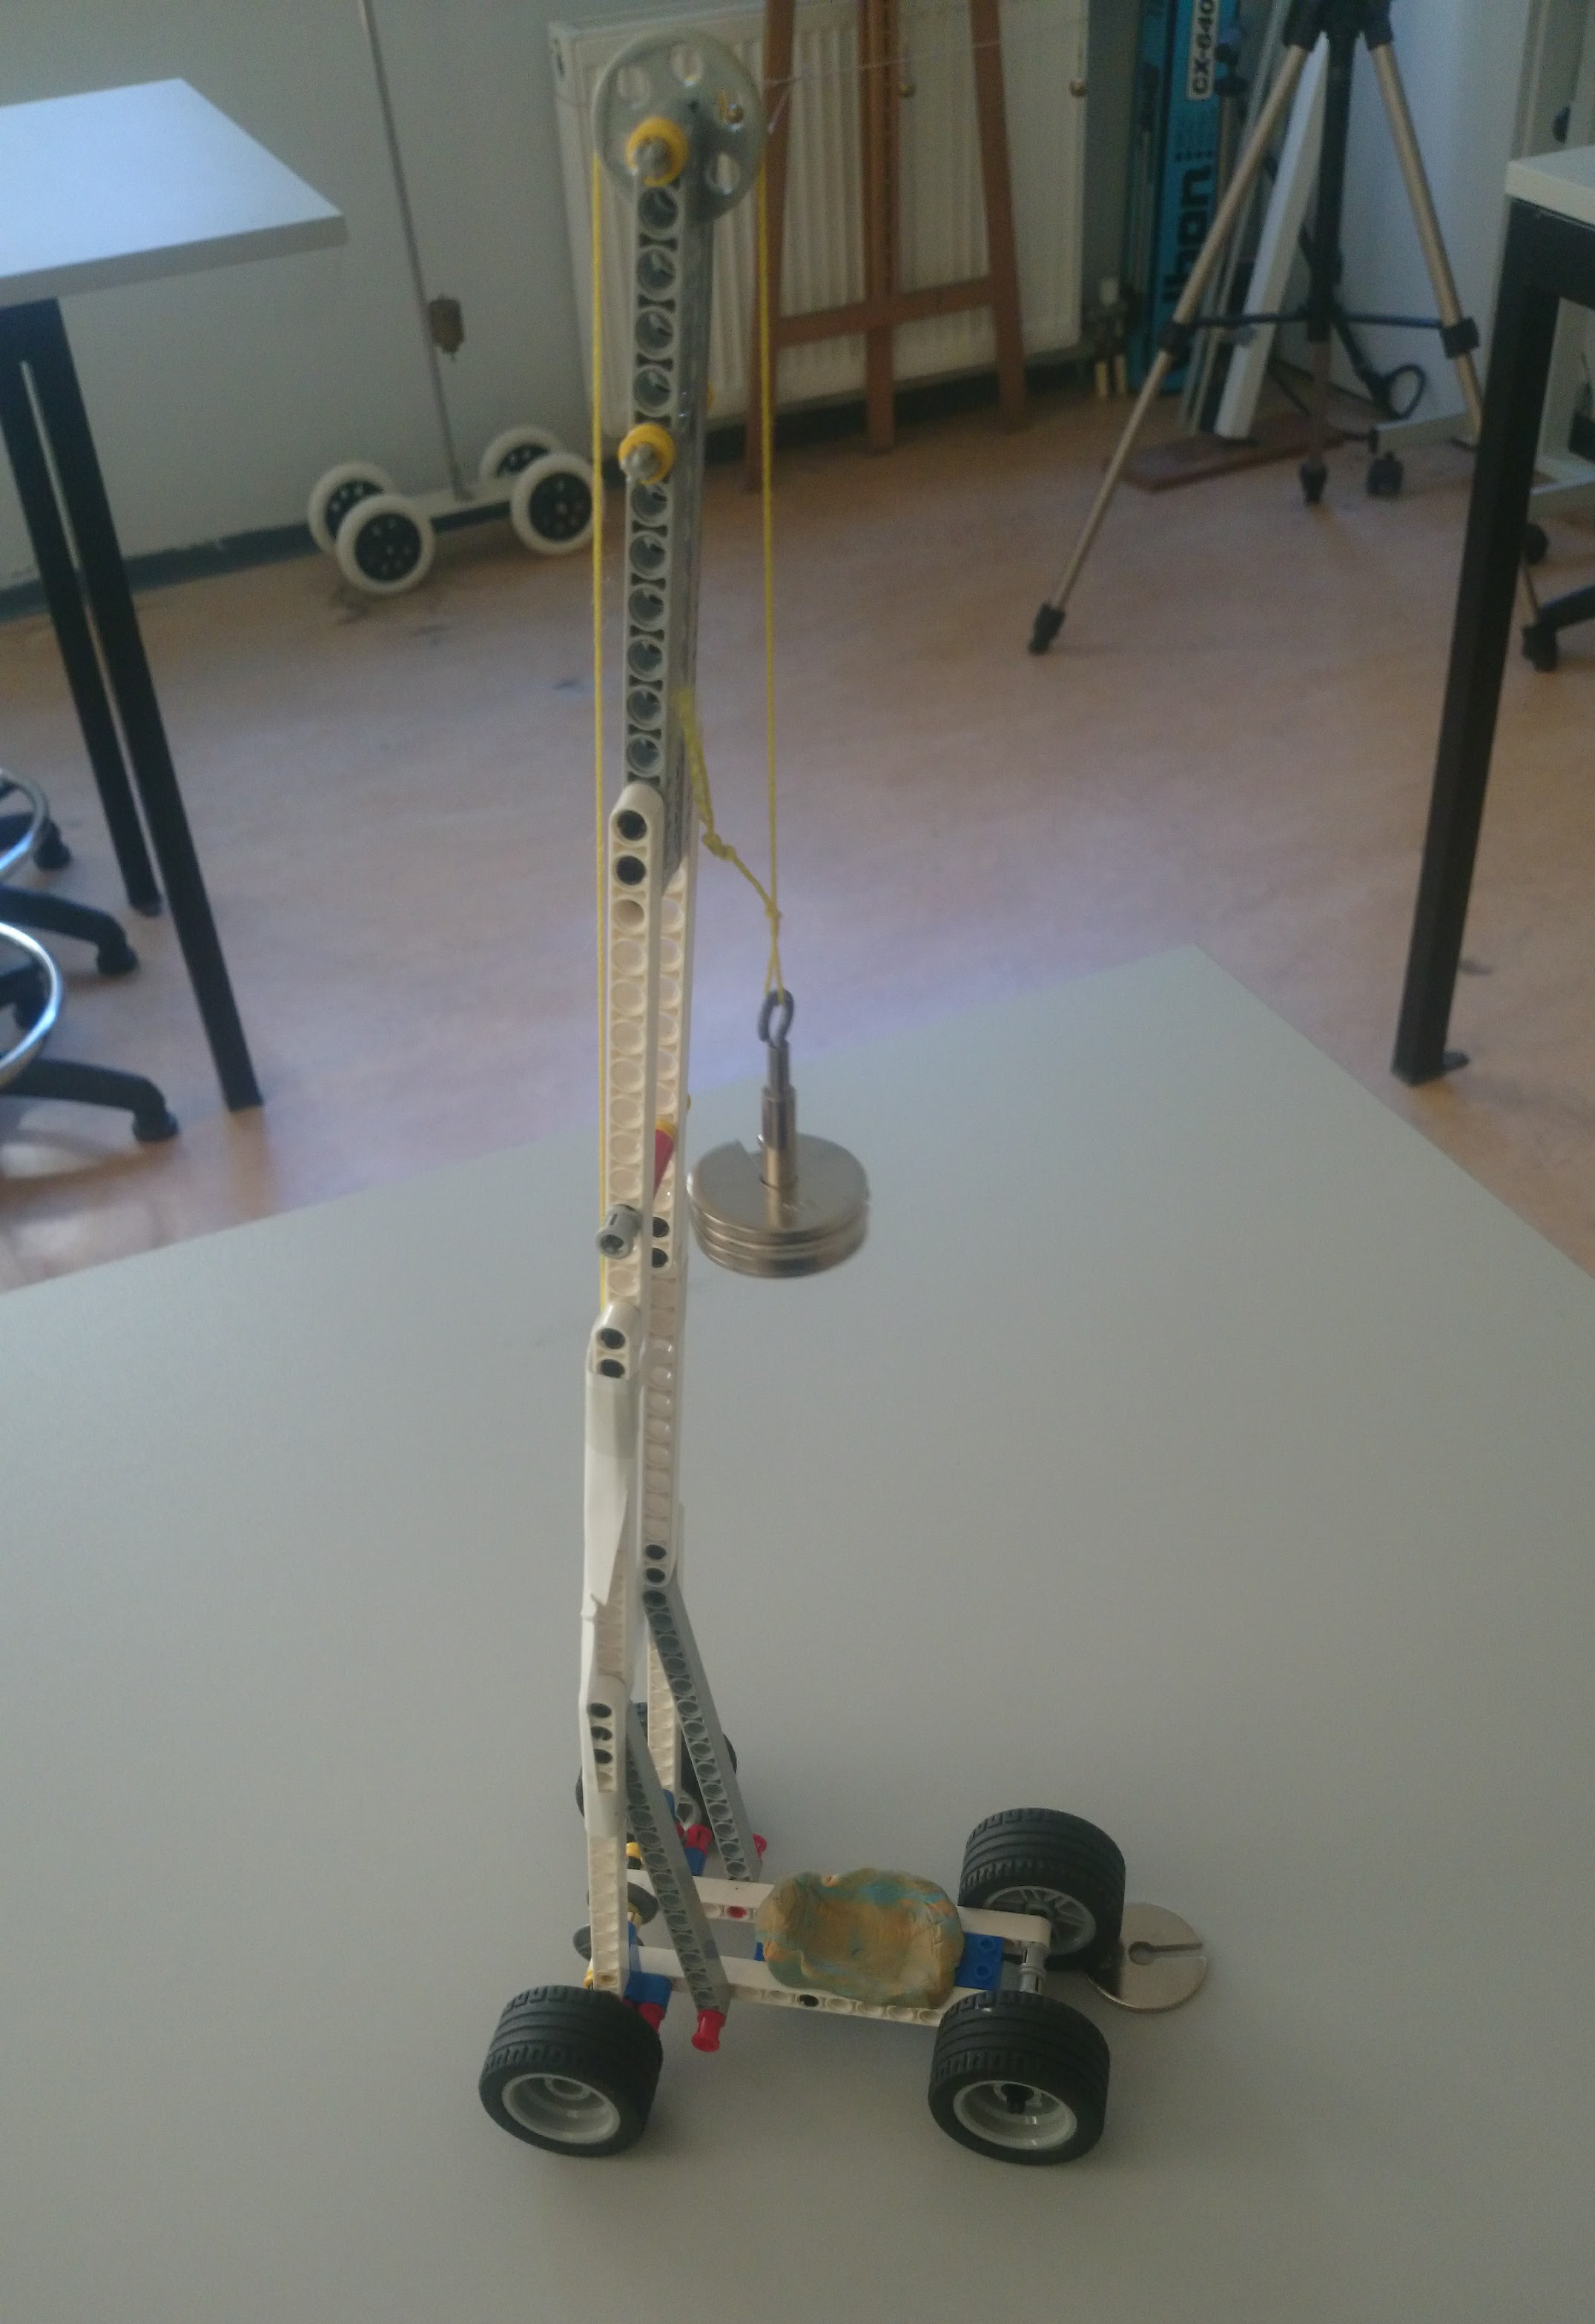
\includegraphics[width=.5\linewidth]{photo_overview.jpg}
        \caption{Picture of gravity car}
        \label{fig:car_picture}
    \end{subfigure}
\end{figure}
%
The car was constructed out of Lego pieces, since they allowed me to make quick changes to
the car until I found an optimal design. \autoref{fig:car_diagram} shows a simplified
diagram of the car, while \autoref{fig:car_picture} is an image of the car that was used for
the experiment.

The measurements of the car will become important in testing the hypothesis on the data and
so they are presented in \autoref{table:car_measurements}:  
%
\begin{table}[H]
    \centering
    \begin{tabular}{l|r}
        Weight of car & 150 g\\
        Height of drop & 35 cm\\
        Weight of wheels & 15 g\\
        Radius of wheels & 2 cm\\
        Radius of axle (at the point where the string is tied) & 5 mm\\
    \end{tabular}
    \caption{}
    \label{table:car_measurements}
\end{table}
    
\subsubsection{Conducting the Experiment}

\begin{enumerate}
    \item Hang weight from string
    \item Roll string on the axis until weight is at the height of the mark
    \item Place car around 40cm from the sensor with an object to prevent it from moving.
        The exact distance does not matter since we are only measuring the distance
        travelled. It must be more than 40 cm, however, since that is the minimum distance
        the sensor can measure.  
    \item Start the logger
    \item Remove the object so the car starts moving
    \item When the car has completely stopped, stop the logger and record the data
\end{enumerate}

\section{Experimental Report}

\subsection{Modifications to the original design}

\begin{itemize}
    \item Because of the weight continuously falling off the car, a small amount of
        plasticine was added to the base of the car shaped in such a way that it would catch
        the weight. (see \autoref{fig:car_base})
        \begin{figure}
            \centering
            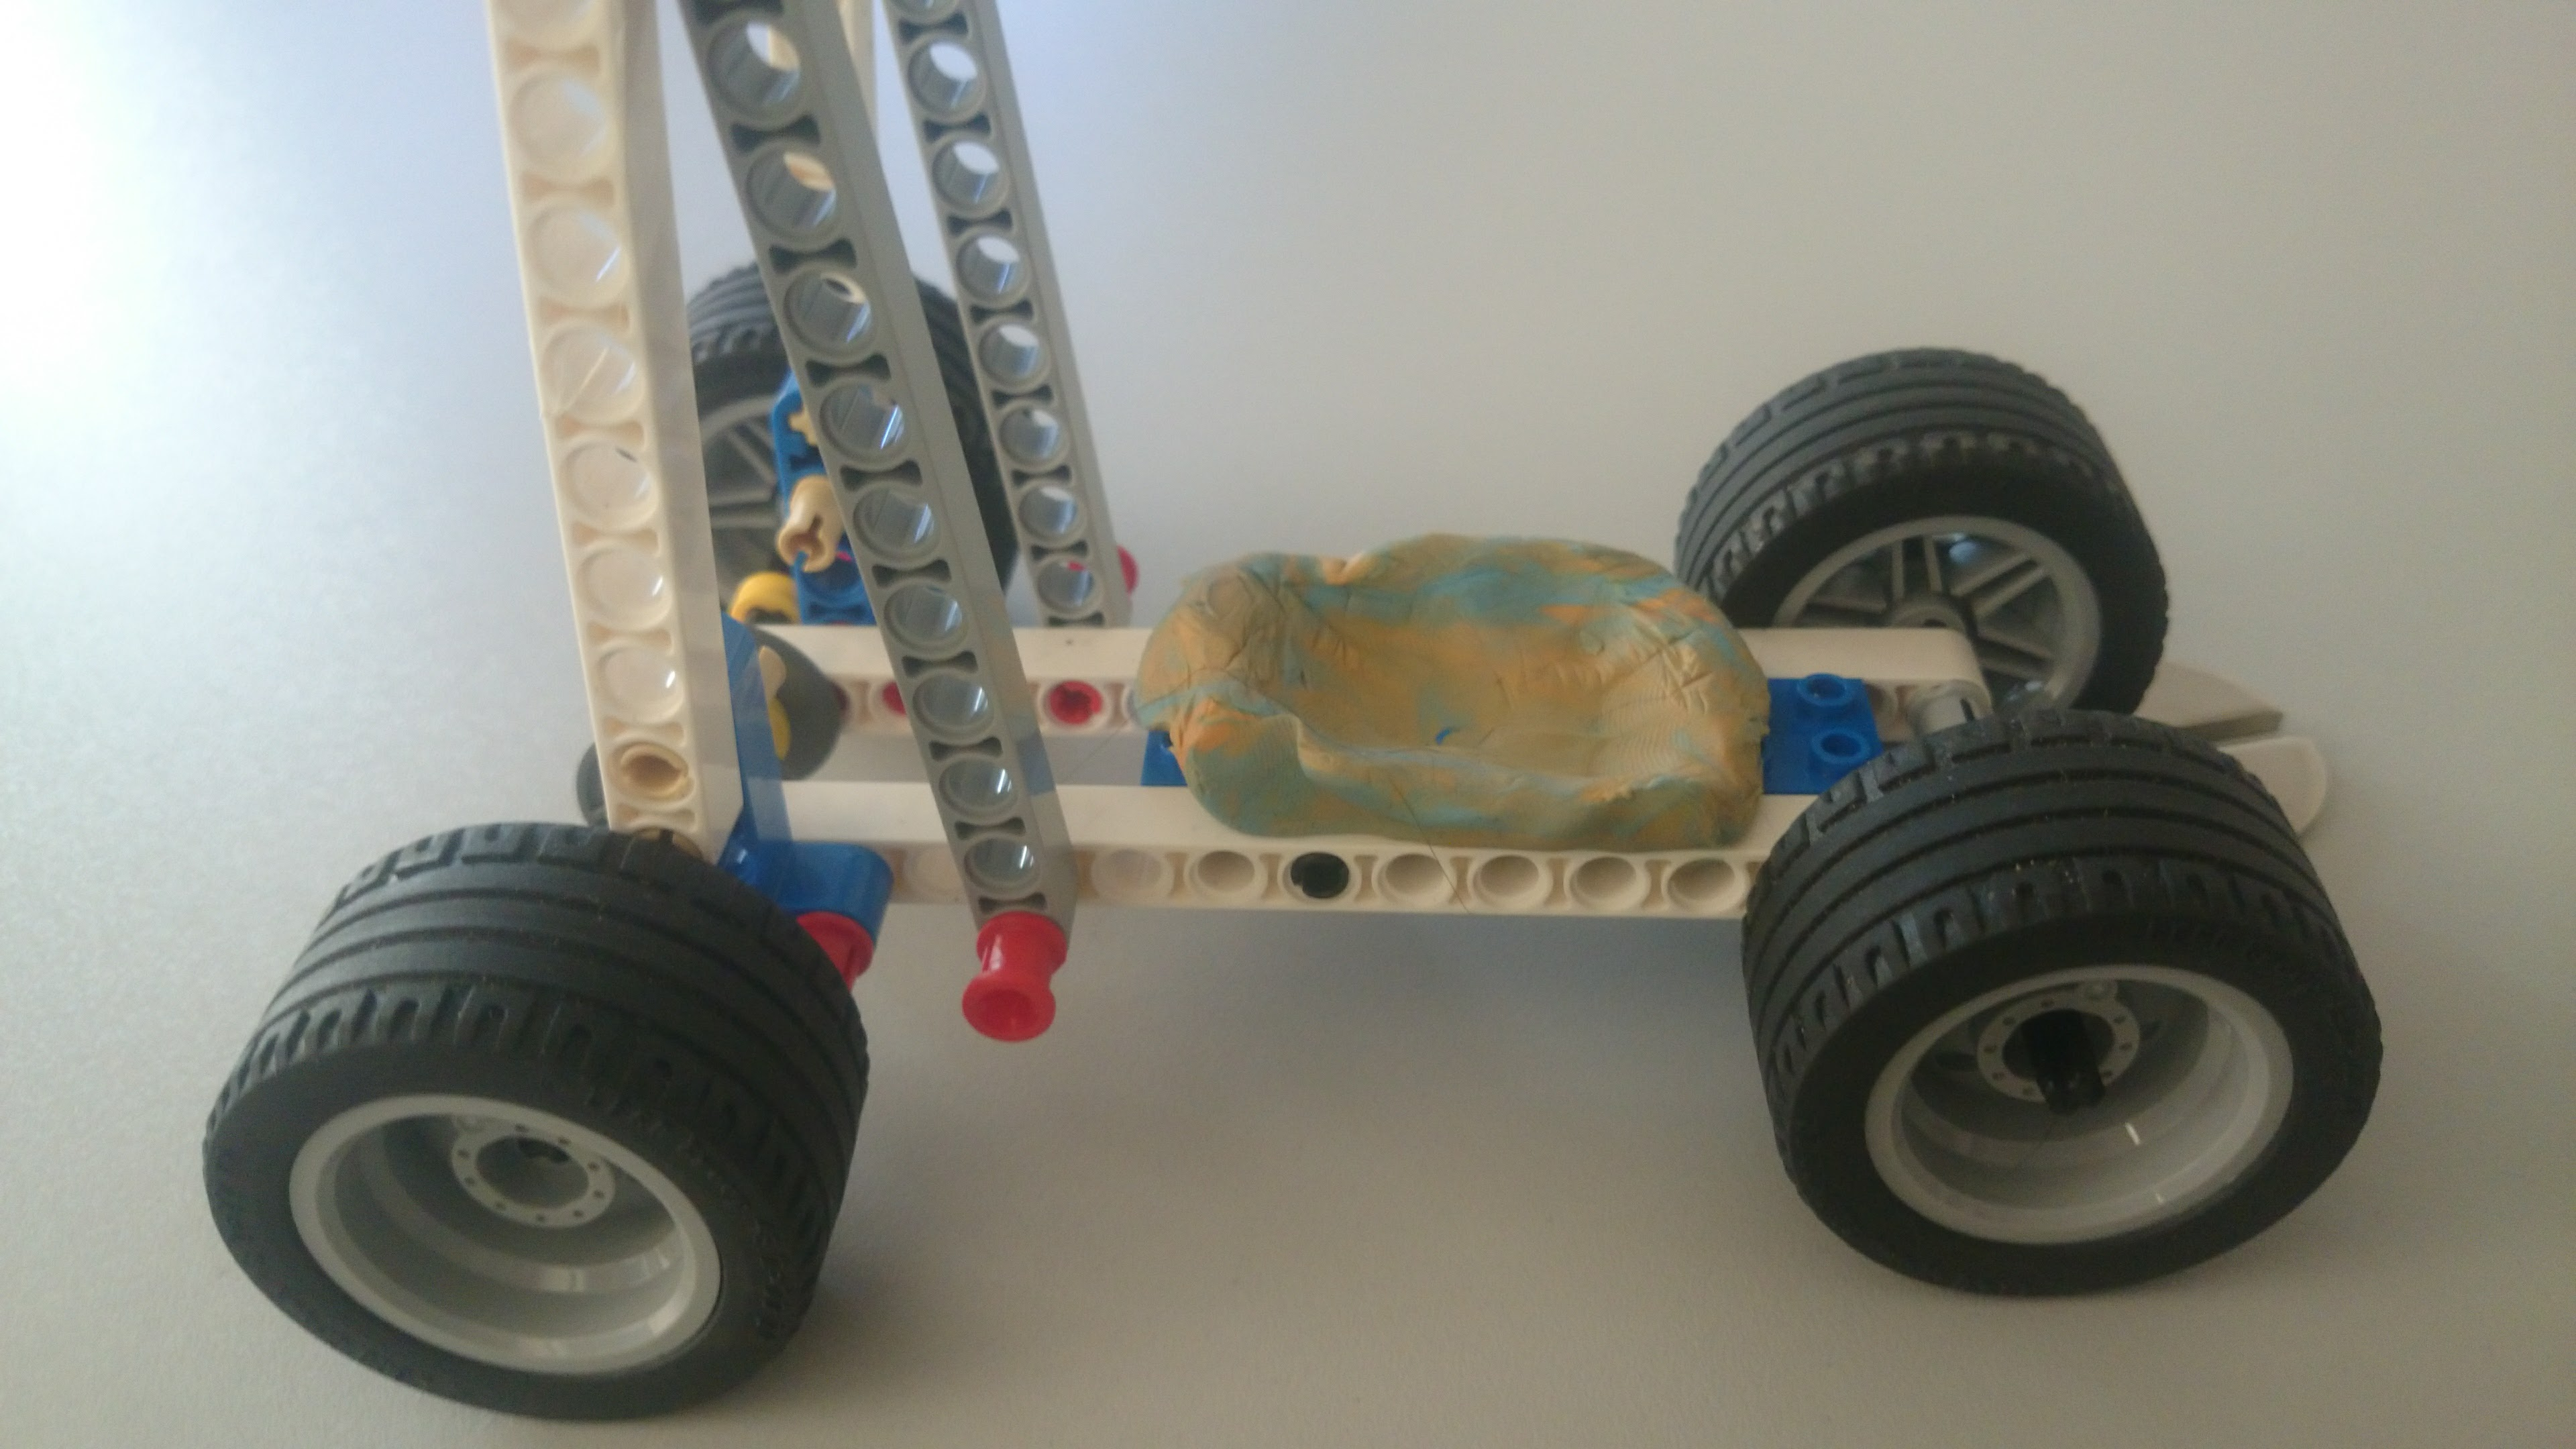
\includegraphics[width=\textwidth]{photo_base.jpg}
            \caption{Plasticine at base of car}
            \label{fig:car_base}
        \end{figure}

    \item When the weight reached the base of the car, the string would start rolling up on
        the axis, stopping the car when it got fully stretched. The solution was to simply
        use a much longer piece of string. This had the side-effect of sometimes getting
        tangled up on the axle, however, all measurements in which that happened were
        discarded.
\end{itemize}

\subsection{Data Collection}

\begin{table}[H]
    \centering
        \def\arraystretch{1.5}
        \begin{tabular}{c|c|c|c|c|c}
            \multirow{2}{*}{mass (kg) $\pm$ 0.0001} & 
                \multicolumn{5}{c}{Distance (m) $\pm$ 0.001}  \\ 
            \cline{2-6}
            & \nth{1} & \nth{2} & \nth{3} & \nth{4} & \nth{5}\\ 
            \hline
            \hline
            0.04 & 1.263 & 1.330 & 1.315 & 1.254 & 1.281\\ 
            \hline
            0.06 & 1.651 & 1.700 & 1.643 & 1.596 & 1.643\\ 
            \hline
            0.08 & 1.858 & 1.922 & 1.920 & 1.935 & 1.905\\ 
            \hline
            0.10 & 1.978 & 1.944 & 1.944 & 1.883 & 1.859\\ 
            \hline
            0.12 & 1.949 & 1.961 & 1.984 & 1.944 & 1.959\\ 
            \hline
            0.14 & 1.972 & 1.969 & 1.971 & 2.023 & 2.021\\ 
            \hline
            0.16 & 2.031 & 2.097 & 2.041 & 2.046 & 2.055\\ 
        \end{tabular}
    \caption{Raw Data} 
    \label{table:raw_data}
\end{table}

\subsection{Data Processing}

\subsubsection{Overview}

For processing the data, I will plot, on the same mass-distance graph, the points
corresponding to each mass tested along with \autoref{eq:s_formula}, to check whether that
line passes through the error bars of each data point.

Since we have five measurements for distance, we will use the arithmetic mean of those five
values. The error of the used value will be calculated as half the difference between the
highest and lowest measurements plus the systematic error of the measurement device
(0.001m), so $\Delta \bar{s} = \frac{1}{2}(s_{max} - s_{min}) + 0.001$. These data will be
plotted on a mass-distance graph, along with \autoref{eq:s_formula}, to demonstrate that it
passes through the error bars of each data point.

Note, that there are no error bars for the mass, since the error in those values is
negligible.

\subsubsection{Presentation}

\FloatBarrier
\begin{table}[H]
    \centering
    \def\arraystretch{1.5}
    \begin{tabular}{c|c|c}
        Mass (kg) & Average & Error\\ 
        \hline
        \hline
        0.04 & 1.289 & 0.0380\\ 
        \hline
        0.06 & 1.647 & 0.0534\\ 
        \hline
        0.08 & 1.908 & 0.0500\\ 
        \hline
        0.10 & 1.922 & 0.0626\\ 
        \hline
        0.12 & 1.959 & 0.0246\\ 
        \hline
        0.14 & 1.991 & 0.0318\\ 
        \hline
        0.16 & 2.054 & 0.0430\\ 
    \end{tabular}
    \caption{Processed Data} 
    \label{table:processed data}
\end{table}

\begin{figure}[H]
    \label{fig:mass-distance-graph}
    \centering
    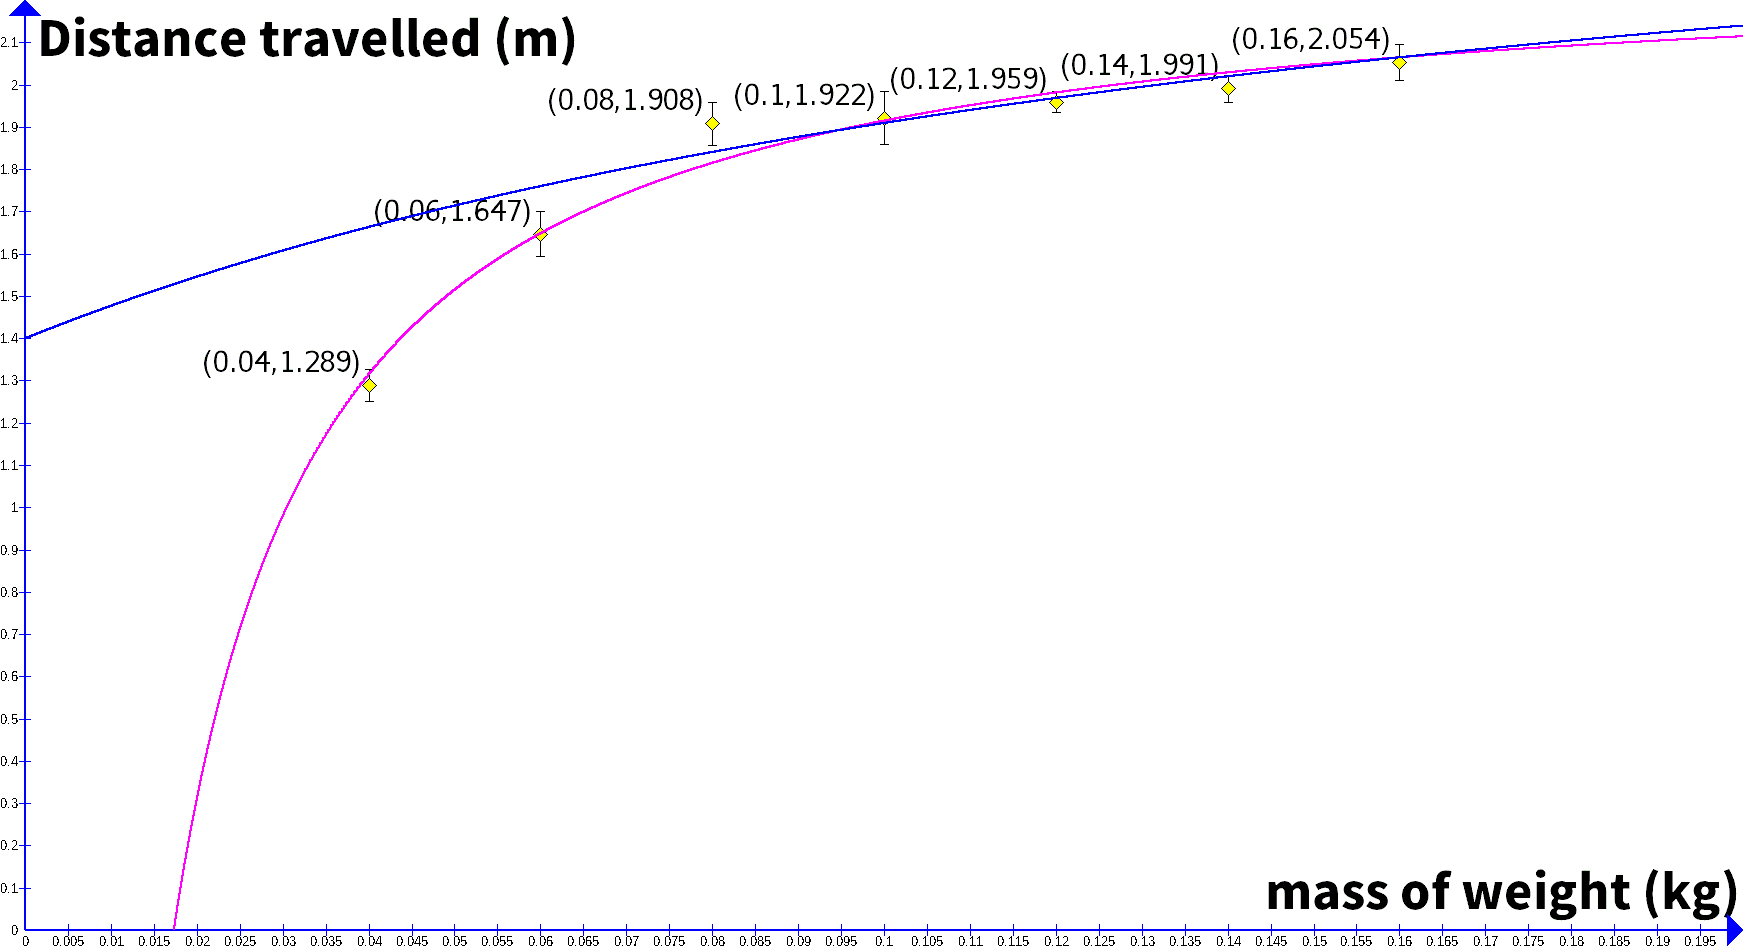
\includegraphics[scale=0.28]{mass-distance_graph}
    \caption{Mass-Distance graph (trendline in pink, 
        \autoref{eq:s_formula} in blue)}
\end{figure}

\FloatBarrier

\subsection{Conclusion \& Evaluation}

\subsubsection{Conclusion \& Justification}

As can be seen from \autoref{fig:mass-distance-graph}, the data seems to support the
hypothesis. The graph of \autoref{eq:s_formula} passes through the error bars of each data
point, suggesting that it correctly models the relationship between the mass attached to the
car and the distance travelled by it. The hypothesis can, therefore, be assumed correct.  

\subsubsection{Evaluating Procedures \& Suggestions for Improvements}

While the data gathered were fairly precise, there was a variety of possible improvements
that could have further increased that precision:

\begin{itemize}
    \item The way that the height from which the weight fell was measured was by having a
        small mark on the tower of the gravity car, and  lining that mark up with the base
        of the weight each time. This method was, of course, very error-prone since lining
        up the weight with the mark was done completely manually. In order to improve the
        consistency of the fall height, a ruler or some other straight object could have
        been used to ensure that the weight fell exactly from the mark each time

    \item The plasticine, while effective in preventing the weight from falling over and
        stopping the car, did introduce another uncertainty into the experiment. On each
        iteration, the fall of the weight would slightly deform the plasticine, meaning that
        on the next iteration, the weight would have a slightly different distance to
        travel, by a few millimeters. 

    \item It was observed after the completion of the experiment that the floor on which the
        experiment was conducted was tilted against the direction on which the car was
        travelling. While this incline did certainly affect the distance that the car
        travelled on each individual measurement, the fact that the incline was constant and
        that the car was, for all measurements, travelling in the same direction, meant that
        it most likely did not affect the overall behaviour of the distance travelled by the
        car relative to the weight used.  
\end{itemize}

\end{document}

